\section{Auswertung}
\label{sec:Auswertung}

\subsection{Bestimmung der Zeitkonstanten durch die Entladnugskurve}

Die bei dem Spannungsabfall des Kondensators gemessenen Wertepaare $(U_\text{c}, T)$ sind in \autoref{tab:entladekurve} zu sehen. 
\begin{table} [h]
  \centering
  \caption{Messdaten zur Entladnugskurve}
  \label{tab:entladekurve}
  \begin{tabular}{c c}
    \toprule
    $U_\text{c} \mathbin{/} \unit{\volt}$ &  $T \mathbin{/} \unit{\micro\second}$ \\
    \midrule
    10,00 &     0 \\
    10,00 &     3 \\
     9,00 &     4 \\
     8,00 &     7 \\
     7,00 &     9 \\
     6,00 &    13 \\
     5,00 &    18 \\
     4,00 &    23 \\
     3,50 &    26 \\
     3,00 &    30 \\
     2,50 &    33 \\
     2,00 &    40 \\
     1,50 &    47 \\
     1,00 &    57 \\
     0,50 &    80 \\
     0,25 &   128 \\
    \bottomrule
    \end{tabular}
\end{table}

Aus diesen Wertepaaren und einer linearen Ausgleichsrechnung wird mittels SCIPY \cite{scipy} die Ausgleichsgerade der Form
\begin{equation*}
  \ln \left(\frac{U_\text{c}}{U_{0}}\right) = - \frac{1}{RC} \cdot t + b
\end{equation*}
in \autoref{fig:plot1} dargestellt.
\begin{figure}[H]
  \centering
  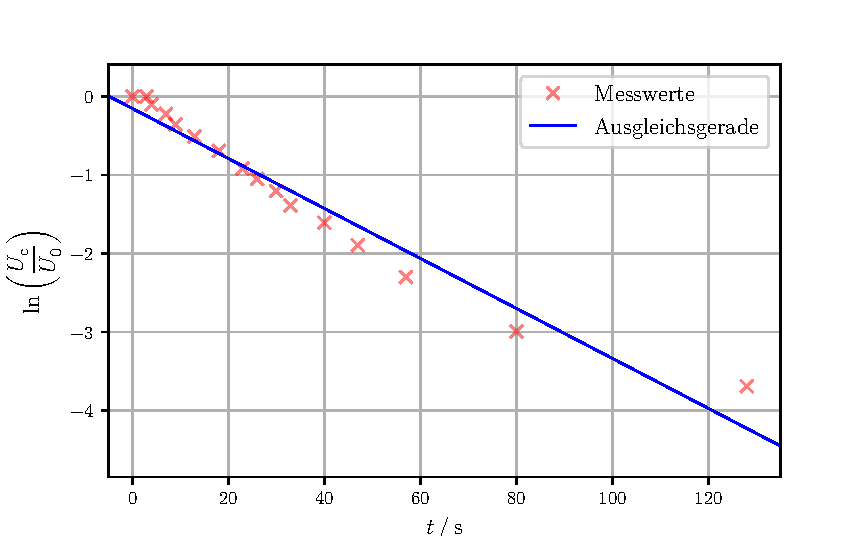
\includegraphics[width=\textwidth]{plot1.pdf}
  \caption{Lineare Ausgleichsgerade zur Bestimmung der Zeitkonstanten mithilfe der Entladekurve.}
  \label{fig:plot1}
\end{figure}

Aus den resultierenden Parametern
\begin{align*}
  a &= \qty[per-mode=reciprocal]{-0.032(002)}{\per\micro\second} \quad \text{und} \\
  b &= (\num{-0.154(083)}) \cdot 10^{-6} \\
  \intertext{ergibt sich nach (\ref{eq:entladung}) für die Zeitkonstante}
  RC &= - \frac{1}{a} = \qty{31.4(1.8)}{\micro\second} \, .
\end{align*}


\subsection{Bestimmung der Zeitkonstanten durch die Frequenz und der anliegenden Wechselspannung}

Die bei den modulierten Frequenzen $f$ gemessene Wechselspannung $U_\text{c}$  sind in \autoref{tab:frequenz} zu sehen. 
\begin{table} [h]
  \centering
  \caption{Messdaten zur Frequenz.}
  \label{tab:frequenz}
  \begin{tabular}{c c c}
    \toprule
    $f \mathbin{/} \unit{\hertz}$ & $U_\text{c} \mathbin{/} \unit{\volt}$ \\
    \midrule
       250 & 5,00 \\
       500 & 4,80 \\
       750 & 4,60 \\
      1000 & 4,60 \\
      1250 & 4,20 \\
      1500 & 4,10 \\
      1750 & 4,00 \\
      2000 & 3,95 \\
      2250 & 3,60 \\
      2500 & 3,30 \\
      2750 & 3,20 \\
      3000 & 3,00 \\
      3250 & 2,80 \\
      3500 & 3,00 \\
      3750 & 2,80 \\
      4000 & 2,75 \\
      6000 & 2,00 \\
      8000 & 1,50 \\
     10000 & 1,20 \\
     20000 & 0,60 \\
     30000 & 0,39 \\
     50000 & 0,25 \\
    100000 & 0,13 \\
    \bottomrule
  \end{tabular}
\end{table}

Aus diesen Werten und einer Ausgleichsrechnung nach (\ref{eq:amp}) wird die Ausgleichsgerade der Form
\begin{equation*}
  \frac{A(\omega)}{U_{0}}=\frac{1}{\sqrt{1+\omega^{2} R^{2} C^{2}}}
\end{equation*}
in \autoref{fig:plot2} dargestellt.
\begin{figure}[H]
  \centering
  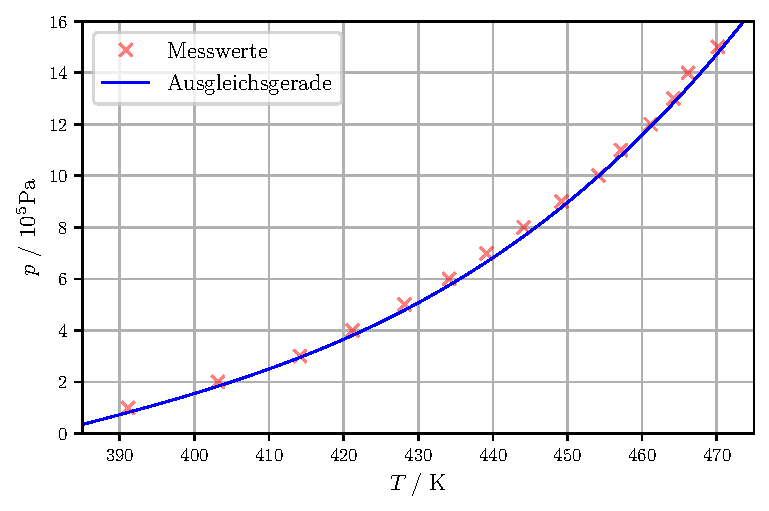
\includegraphics[width=\textwidth]{plot2.pdf}
  \caption{Ausgleichsrechnung zur Bestimmung der Zeitkonstanten mithilfe der Frequenz.}
  \label{fig:plot2}
\end{figure}
Darus ergibt sich nun die Zeitkonstante zu
\begin{equation*}
  RC = \qty{-66.7(1.2)}{\micro\second} \, .
\end{equation*}


\subsection{Bestimmung der Zeitkonstanten durch die Phasenverschiebung}

Die Bestimmung der Phasenverschiebung zischen Generatorspannung und Kondensatorspannung erfolgt mithilfe der Messwerte in \autoref{tab:dt}.
\begin{table} [h]
  \centering
  \caption{Messdaten zur Phasenverschiebung.}
  \label{tab:dt}
  \begin{tabular}{c c c}
    \toprule
    $f \mathbin{/} \unit{\hertz}$ & $U_\text{c} \mathbin{/} \unit{\volt}$ & $\phi \mathbin{/} \mathrm{rad}$ \\
    \midrule
       250 &   5 &   0,0628 \\
       500 &   5 &   0,1257 \\
       750 &   5 &   0,1885 \\
      1000 &   5 &   0,1759 \\
      1250 &   4 &   0,1649 \\
      1500 &   4 &   0,1885 \\
      1750 &   4 &   0,2199 \\
      2000 &   4 &   0,2513 \\
      2250 &   4 &   0,2827 \\
      2500 &   3 &   0,3142 \\
      2750 &   3 &   0,3283 \\
      3000 &   3 &   0,3581 \\
      3250 &   3 &   0,3676 \\
      3500 &   3 &   0,3738 \\
      3750 &   3 &   0,4006 \\
      4000 &   3 &   0,4273 \\
      6000 &   2 &   0,4524 \\
      8000 &   2 &   0,5027 \\
     10000 &   1 &   0,5027 \\
     20000 &   1 &   0,7540 \\
     30000 &   0 &   0,3770 \\
     50000 &   0 &   0,6283 \\
    100000 &   0 &   0,6283 \\
    \bottomrule
  \end{tabular}
\end{table}

Aus diesen Werten und einer Ausgleichsrechnung nach (\ref{eq:phase}) wird die Ausgleichsgerade der Form
\begin{equation*}
  \phi=a \arctan (b x)
\end{equation*}
in \autoref{fig:plot3} dargestellt.
\begin{figure}[H]
  \centering
  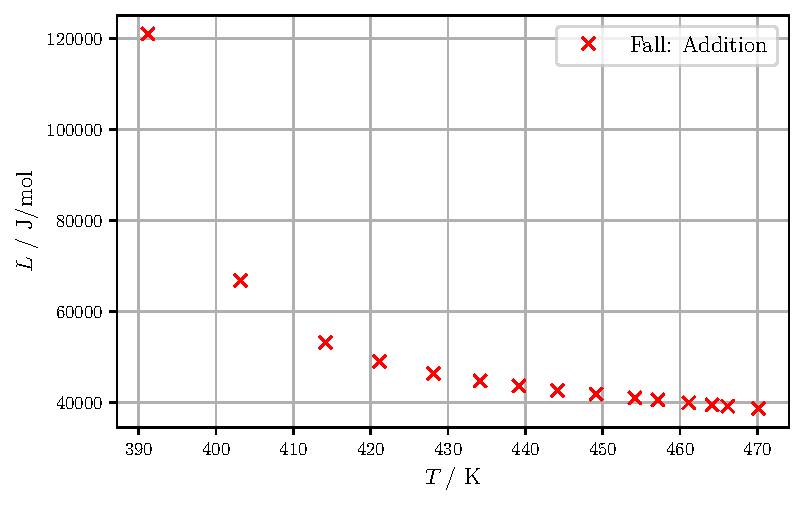
\includegraphics[width=\textwidth]{plot3.pdf}
  \caption{Ausgleichsrechnung zur Bestimmung der Zeitkonstanten mithilfe der Phasenverschiebung.}
  \label{fig:plot3}
\end{figure}
Darus ergibt sich nun die Zeitkonstante zu
\begin{equation*}
  RC = \qty{4.5(1.2)}{\micro\second} \, .
\end{equation*}

Es wird des Weiteren zur besseren Veranschaulichung ein Polarplot in \autoref{fig:plot4} dargestellt.
\begin{figure}[H]
  \centering
  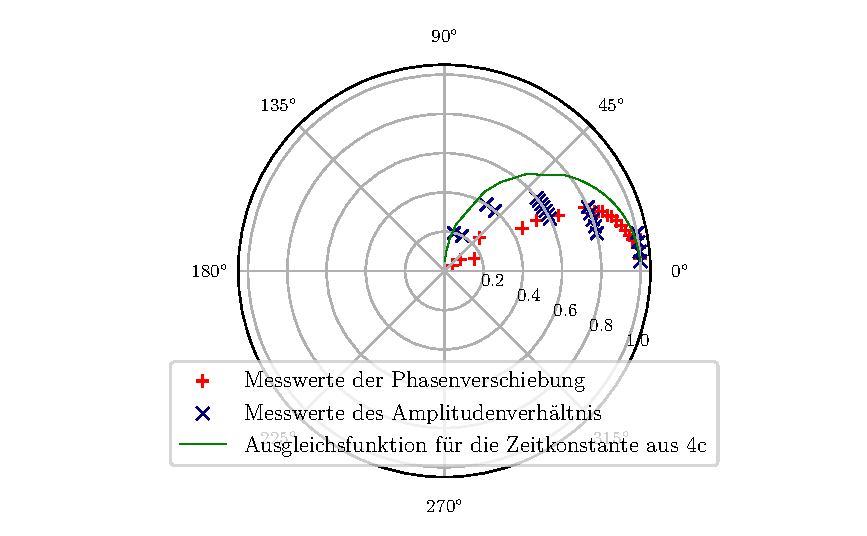
\includegraphics[width=\textwidth]{plot4.pdf}
  \caption{Polarplot zur Beobachtung der Phasenverschiebung zwischen der Generator und Kondensatorspannung.}
  \label{fig:plot4}
\end{figure}

Um die Integrierbarkeit der RC-Spannung zu zeigen, wird der Erwartungswert mit dem
Realwert vom Oszilloskop verglichen. Da sich Erwartungs- und Realwert decken ist gezeigt
das die RC Spannung integrabel ist.
\begin{figure}[H]
  \centering
  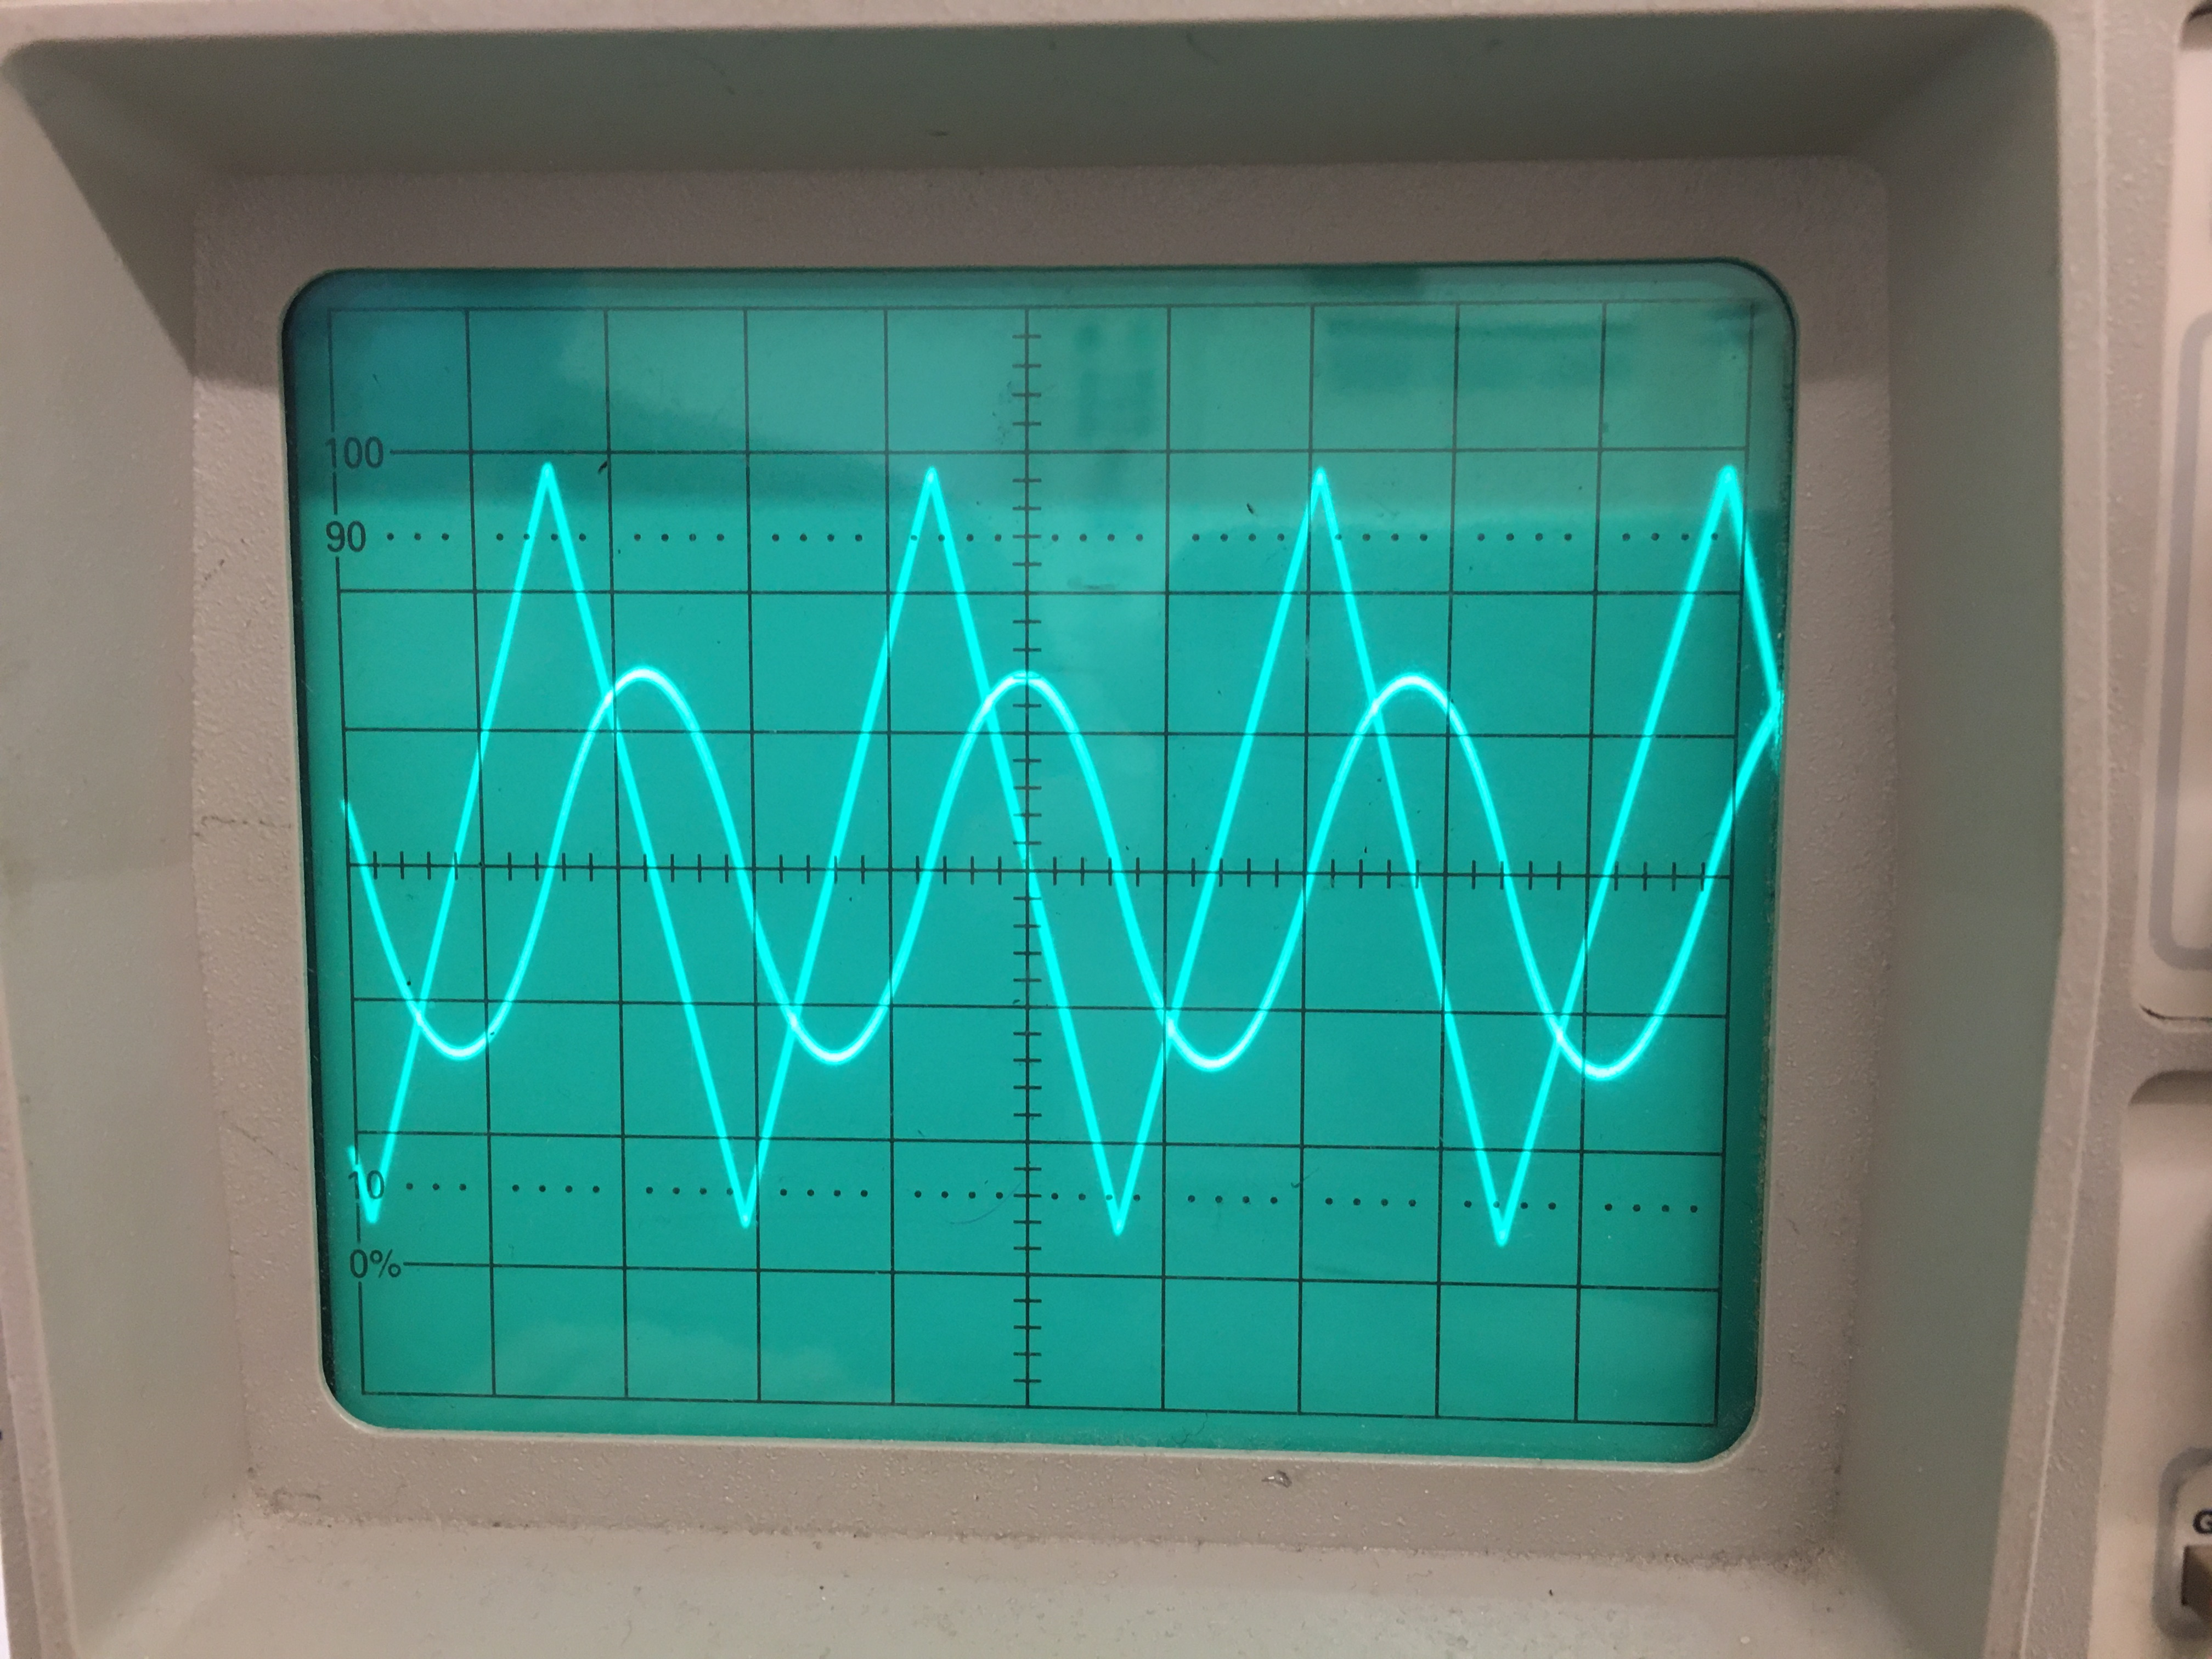
\includegraphics[width=0.8\textwidth]{pictures/dreieck.jpg}
  \caption{Dreiecksspannung integriert.}
  \label{fig:dreieck}
\end{figure}